\documentclass[12pt]{article}
\usepackage[a4paper, total={7.5in, 10.5in}]{geometry}
\usepackage{array}
\usepackage{graphicx, subfig, wrapfig, fancyhdr, lastpage, multicol ,color,arydshln,makecell}
\newcommand\headerMe[2]{\noindent{}#1\hfill#2}
\usepackage[mathscr]{euscript}
\usepackage{tabularray}

\setlength{\columnseprule}{1pt}
\def\columnseprulecolor{\color{blue}}


\pagestyle{fancy}
\fancyhf{}

\cfoot{\vspace{-1cm}\em{Page \thepage \hspace{1pt} / \pageref{LastPage}}}
\begin{document}

\headerMe{Royaume du Maroc}{année scolaire \emph{2024-2025}}\\
\headerMe{Ministère de l'Éducation nationale, }{  Professeur :\emph{Zakaria Haouzan}}\\
\headerMe{du Préscolaire et des Sports}{Établissement : \emph{Lycée SKHOR qualifiant}}\\
%\vspace{-1cm}
\begin{center}
	Devoir Surveillé  N°2 \\
	2ème année baccalauréat Sciences physiques\\
	Durée 2h00
	\\
	\vspace{.2cm}
	\hrulefill
	\Large{Chimie 7pts - 45min}
	\hrulefill\\

\emph{Transformations non totales d'un système chimique\dotfill(7pts)-45min }
\end{center}
%end Headerss------------------------
%__________________Chimie ______________________-
%%%%%%%+_+_+_+_+_+_+_+_+_Partie1

%\begin{wrapfigure}{r}{0.16\textwidth}
%\vspace{-1.2cm}
%%\begin{center}
%%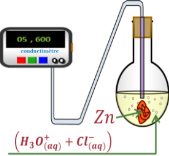
\includegraphics[width=0.16\textwidth]{./img/chimie01.png}
%%\end{center}
%\end{wrapfigure}


%\begin{wrapfigure}[1]{r}{0.5\textwidth}
%\vspace{0.5cm}
%\begin{center}
%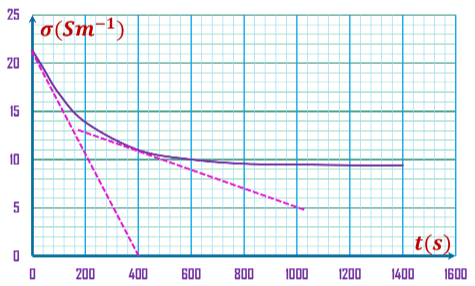
\includegraphics[width=0.5\textwidth]{./img/chimie02.png}
%\end{center}
%\end{wrapfigure}

\emph{L’acide méthanoïque HCOOH, couramment appelé acide formique, est un liquide
	piquant et corrosif qui existe à l’état naturel dans l’organisme des fourmis rouges.
	Cet exercice vise :}
\begin{itemize}
	\item  L’étude d’une solution aqueuse d’acide méthanoïque,
	\item  L’étude de l’effet de la dilution sue le taux d’avancement final $\tau$.
\end{itemize}

\section*{Partie 1 : Etude d’une solution aqueuse d’acide méthanoïque.\\\dotfill(2,5pts) }

On dispose d’une solution aqueuse $(S_1)$ d’acide méthanoïque HCOOH de volume de
$V_1= 500mL$ concentration molaire $C_1 = 0,10 mol.L^{-1}$ et de $pH_1=2,4$.

\begin{tabular}{c|l}
	0,25 & \makecell[l]{\textbf{1. }Définir un acide selon Bronsted.}                                                  \\
	0,25 & \makecell[l]{\textbf{2. }Ecrire l’équation modélisant la dissolution de l’acide éthanoïque dans l’eau.}     \\
	0,75 & \makecell[l]{\textbf{3. }Calculer la valeur de l’avancement final $x_f$ de cette réaction. }                \\
	0,75 & \makecell[l]{\textbf{4. }Calculer la valeur du taux d’avancement final $\tau_1$ de cette réaction. Conclure.} \\
	0,5  & \makecell[l]{\textbf{5. }Déterminer la constante d’équilibre $K_1$ de cette réaction.}
\end{tabular}

\section*{Partie 2 : L’étude de l’effet de la dilution sue le taux d’avancement final.\dotfill(4,5pts)}

On prend un volume de la solution précédente $(S_1)$ et on y ajoute une quantité d’eau
distillée pour obtenir une solution aqueuse $(S_2)$ d’acide méthanoïque de concentration
$C_2 = 5.10^{-3} mol.L^{-1}$ et de volume $V_2$. La mesure de la conductivité de la solution $(S_2)$ a donné la valeur $\sigma_{eq} = 3,5.10^{-2} S.m^{-1}$.

\begin{itemize}
  \item  Les conductivités molaires ioniques :\\ 
    $\lambda_1 = \lambda_{H_3O^+}$=$3,49.10^{-2}S.m^2/mol$ ; $\lambda_2 = \lambda_{HCOO^-}$=$4,09.10^{-3}S.m^2/mol$
\end{itemize}

\begin{tabular}{c|l}
  0,5 & \makecell[l]{ \textbf{1. }Exprimer la conductivité $\sigma_{eq}$ de la solution en fonction de $\lambda_1$, $\lambda_2$ et  $[H_3O^+]_{eq}$ la concentration \\effective des ions oxonium à l’état final. }        \\

  0,5 & \makecell[l]{\textbf{2. }Montrer que $[H_3O^+]_{eq} = \frac{\sigma_{eq}}{\lambda_1 + \lambda_2}$ puis calculer sa valeur.}\\

	0,75 & \makecell[l]{\textbf{3. }En déduire la valeur $pH_2$ de la solution $S_2$ . Comparer $pH_1$ et $pH_2$ puis en déduire l’effet de \\la dilution sur le pH de la solution.} \\

	0,25 & \makecell[l]{\textbf{4. }Calculer la valeur du taux d'avancement final $\tau_2$ dans ce cas.}                                               \\

1 & \makecell[l]{\textbf{5. }Déterminer la valeur de $K_2$.}                     \\

	1,5 & \makecell[l]{\textbf{6. }Comparer les valeurs de $\tau_1$ et $\tau_2$ .En déduire l’effet de la dilution sur le taux \\d’avancement final et la constance d’équilibre.}

\end{tabular}
%\hrulefill
%\Large{Physique 13pts/78min}
%\hrulefill\\
\newpage

	\vspace{-1cm}
\begin{center}
	\hrulefill
	\Large{Physique 13pts - 75min}
	\hrulefill\\
	\emph{ La radioactivité au service de la médecine}
\end{center}

\vspace{-1cm}
%\vspace{-1cm}
\section*{Partie 1: L'étude d'un nucléide d'azote 13.\dotfill(6pts)}

%\begin{wrapfigure}[2]{r}{0.19\textwidth}
%\begin{center}
%\vspace{-2cm}
%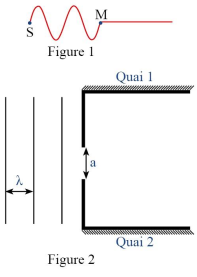
\includegraphics[width=0.19\textwidth]{./img/ex6.png}
%\end{center}
%\end{wrapfigure}

\vspace{-0.2cm}
L'azote 13 est un isotope radioactif, utilisé dans le traitement des maladies pulmonaires et dans l'imagerie du flux sanguin dans le muscle cardiaque.

La désintégration du nucléide d'azote $^{13}_7N$ produit un nucléide de carbone $^{13}_6C$.


\begin{tabular}{c|l}

	1 & \makecell[l]{\textbf{1.1. } Écrire l'équation de désintégration et déterminer le type de la particule émise.} \\
	0,75 & \makecell[l]{\textbf{1.2. } Donner la composition du noyau d'azote 13.} \\
	0,5 & \makecell[l]{\textbf{1.3. } Calculer l'énergie de liaison d'un noyau d'azote 13. } \\
	0,5 & \makecell[l]{\textbf{1.4. } Déduire l'énergie de liaison par nucléon du noyau d'azote 13. } \\
	0,25 & \makecell[l]{\textbf{1.5. } L'énergie de liaison par nucléon du carbone 13 est $\xi_C = 7,466$ MeV/nucléon.\\ Déterminer le noyau le plus stable parmi les noyaux $^{13}_7N$ et $^{13}_6C$.} \\
\end{tabular}

1.6.Le noyau d'azote 13 est produit par une réaction entre le noyau d'oxygène 16 et un proton rapide selon l'équation suivante : 
    $
    ^{16}_8O + ^{1}_1P \rightarrow ^{13}_7N + ^{A}_Z X
    $

\begin{tabular}{c|l}
	1 & \makecell[l]{\textbf{1.6.a. } En appliquant les lois de conservation, déterminer les nombres $A$ et $Z$ puis identifier le noyau.
} \\
	2 & \makecell[l]{\textbf{1.6.b. } Calculer en MeV l'énergie $\Delta E$ produite par cette réaction nucléaire. \\Cette réaction est-elle exoénergétique ou endoénergétique ?
} \\

\end{tabular}

\section*{Données :}
\vspace{-1.4cm}
\begin{center}
\begin{tabular}{|c|c|c|}
\hline
$m(^{13}N) = 13,00574 u$ & $1 u = 931,5 MeV.c^{-2}$ & $t_{1/2}(^{14}C) = 5700 ans$ \\\hline
$m_p = 1,00728 u$ & $m(^{16}O) = 15,9905u $ & $N_A = 6,02.10^{23}.mol^{-1}$ \\\hline
$m_n = 1,00866 u$ & $m(^AX) = 4,0015 u$ & $M(^{14}C) = 14 g/mol$ \\\hline
\end{tabular}
\end{center}
\section*{Partie 2: datation par le carbone 14.\dotfill(3pts)}

Dans une grotte préhistorique, on a trouvé un morceau de bois fossilisée contenant une masse $m = 2.10^{-12} g$ de carbone 14.

Un autre morceau de même masse, coupé récemment d'un arbre, contient une masse $m_0 = 9 \cdot 10^{-12} g$ de carbone 14.



\begin{tabular}{c|l}

	0,75   & \makecell[l]{\textbf{2.1 } Quelle est la signification physique du temps de demi-vie $t_{1/2}$ ?
}\\
	0,75   & \makecell[l]{\textbf{2.2 } Calculer l'activité radioactive à l'origine de ce morceau de bois.}\\
	1,5   & \makecell[l]{\textbf{2.3 } En s'appuyant sur la loi de la désintégration radioactive, montrer que l'expression de l'âge \\du morceau de bois s'écrit :
    $
    t = \frac{t_{1/2}}{\ln 2} \cdot \ln (\frac{m_0}{m})
    $
    Calculer sa valeur en années.
}\\

	\end{tabular}


\section*{Partie 3:  Etude d’un stimulateur cardiaque\dotfill(4pts)}
Le stimulateur cardiaque est un appareil médical introduit par chirurgie à l’intérieur du corps
humain qui souffre d’une insuffisance cardiaque Cet appareil fonctionne avec une batterie qui utilise
l’énergie nucléaire produit par la réaction de désintégration du noyau du plutonium $Pu$.
\begin{center}

\begin{tabular}{ |c|c|c|c|c| }
	\hline
Le noyau & $^A_ZX$ & $^{240}_{94}Pu$ & $^{238}_{94}Pu$ & $^{234}_{92}U$\\\hline
L’énergie de liaison EL en MeV &
28,285 &1813,008 &1800,827& 1778,142\\\hline
La demi- vie (ans)&
				  &  & 87,7&  \\\hline
\end{tabular}
\end{center}

\begin{tabular}{c|l}
  1 & \makecell[l]{\textbf{1. } Le plutonium a des isotopes tel que $^{240}_{94}Pu$ et $^{238}_{94}Pu$ . Déterminer le noyau le plus stable.}\\
\end{tabular}

  2. La désintégration du plutonium $^{238}_{94}Pu$ conduit à la formation du noyau d’uranium $^{234}_{92}U$ avec
émission d’une particule $^A_ZX$.


\begin{tabular}{c|l}
  1 & \makecell[l]{\textbf{2.1 } Ecrire l’équation de désintégration du noyau du plutonium $^{238}_{94}Pu$ et déterminer la nature\\ de la
particule émise.}\\

  1 & \makecell[l]{\textbf{2.2. } Trouver en MeV l’énergie libérée $E_{lib}$ durant la désintégration d’un noyau du plutonium $238$.}\\

  1 & \makecell[l]{\textbf{3. } A l’instant $t=0$ on introduit à un malade de 40 ans un stimulateur cardiaque. Le cœur du \\malade
fonctionne normalement jusqu’ à ce que l’activité du plutonium contenu dans le stimulateur
\\devient $a=0,7a_0$, avec $a_0$ l’activité a l’instant $t = 0$. \\Déterminer l’âge du malade lorsqu’on change
le stimulateur cardiaque}\\
\end{tabular}
\end{document}
